% questions.tex —— 1986 年·全国卷·文科 · 题目内容片段（无答案）
% 由 tools/generate_projects.py 依来源总账自 1986/1986_数学真题_全国文_试题.md 生成，勿手改（改源 MD 后重跑）


\gkpart{文科数学}

\begin{gktip}
\textbf{来源说明}：本题面依据固定源 PDF《1986 年普通高等学校招生考试（全国卷）·文科数学》单页逐题转录。固定源原卷页码为 28；该 PDF 不含答案页，下列答案和解析由本库独立推导，不声称代表官方发布版本。

\textbf{图形说明}：第 10 题的四个函数图象选项和第 17 题的立体图形均依据固定源图形关系重绘为 TikZ 矢量图。
\end{gktip}

\begin{question}
\gkti{1}在下列各数中，已表示成三角形式的复数是\mbox{（　　）}

（A）$2\left(\cos\frac\pi4-i\sin\frac\pi4\right)$

（B）$2\left(\cos\frac\pi4+i\sin\frac\pi4\right)$

（C）$2\left(\sin\frac\pi4+i\cos\frac\pi4\right)$

（D）$-2\left(\sin\frac\pi4-i\cos\frac\pi4\right)$

\end{question}
\begin{question}
\gkti{2}函数

\nopagebreak[4]
\[
y=5^x+1
\]

的反函数是\mbox{（　　）}

（A）$y=\log_5(x+1)$　　（B）$y=\log_x5+1$

（C）$y=\log_5(x-1)$　　（D）$y=\log_{x-1}5$

\end{question}
\begin{question}
\gkti{3}已知全集 $I=\{1,2,3,4,5,6,7,8\}$，$A=\{3,4,5\}$，$B=\{1,3,6\}$，那么集合 $\{2,7,8\}$ 是\mbox{（　　）}

（A）$A\cup B$　　（B）$A\cap B$　　（C）$\overline A\cup\overline B$　　（D）$\overline A\cap\overline B$

\end{question}
\begin{question}
\gkti{4}函数

\nopagebreak[4]
\[
y=\sqrt2\sin2x\cos2x
\]

是\mbox{（　　）}

（A）周期为 $\dfrac\pi2$ 的奇函数　　（B）周期为 $\dfrac\pi2$ 的偶函数

（C）周期为 $\dfrac\pi4$ 的奇函数　　（D）周期为 $\dfrac\pi4$ 的偶函数

\end{question}
\begin{question}
\gkti{5}已知 $c>0$，在下列不等式中成立的一个是\mbox{（　　）}

（A）$c>2^c$　　（B）$c>\left(\dfrac12\right)^c$

（C）$2^c<\left(\dfrac12\right)^c$　　（D）$2^c>\left(\dfrac12\right)^c$

\end{question}
\begin{question}
\gkti{6}有以下 20 个数：

\nopagebreak[4]
\[
87,\ 91,\ 94,\ 88,\ 93,\ 91,\ 89,\ 87,\ 92,\ 86,\ 90,\ 92,\ 88,\ 90,\ 91,
86,\ 89,\ 92,\ 95,\ 88,
\]

它们的和是\mbox{（　　）}

（A）1789　　（B）1799　　（C）1879　　（D）1899

\end{question}
\begin{question}
\gkti{7}已知某正方体对角线长为 $a$，那么这个正方体的全面积是\mbox{（　　）}

（A）$2\sqrt2a^2$　　（B）$2a^2$　　（C）$2\sqrt3a^2$　　（D）$3\sqrt2a^2$

\end{question}
\begin{question}
\gkti{8}如果方程

\nopagebreak[4]
\[
x^2+y^2+Dx+Ey+F=0\ (D^2+E^2-4F>0)
\]

所表示的曲线关于直线 $y=x$ 对称，那么必有\mbox{（　　）}

（A）$D=E$　　（B）$D=F$　　（C）$E=F$　　（D）$D=E=F$

\end{question}
\begin{question}
\gkti{9}设甲是乙的充分条件，乙是丙的充要条件，丙是丁的必要条件，那么丁是甲的\mbox{（　　）}

（A）充分条件　　（B）必要条件　　（C）充要条件　　（D）既不充分也不必要的条件

\Needspace{0.4\textheight}
\end{question}
\begin{question}
\gkti{10}在下列各图中，$y=ax^2+bx$ 与 $y=ax+b$（$ab\ne0$）的图象只可能是\mbox{（　　）}
\nopagebreak[4]
\begin{center}% 1986 年全国卷文科第 10 题：四个函数图象选项
\begin{tikzpicture}[scale=0.72,>=stealth]
  \foreach \dx/\dy/\lab/\curve/\line in {
    0/2.25/{（A）}/{1.55*(\x+0.45)^2-0.55}/{0.85*\x+0.55},
    3.15/2.25/{（B）}/{1.55*\x*\x-1.55*\x}/{-0.85*\x+0.80},
    0/0/{（C）}/{-1.45*\x*\x+1.45*\x}/{-0.72*\x+0.85},
    3.15/0/{（D）}/{-1.45*\x*\x+1.45*\x}/{0.72*\x-0.55}
  } {
    \begin{scope}[shift={(\dx,\dy)}]
      \draw[->] (-1.35,0)--(1.45,0) node[right] {$x$};
      \draw[->] (0,-1.35)--(0,1.45) node[above] {$y$};
      \draw[thick,domain=-1.15:1.15,samples=80]
        plot (\x,{\curve});
      \draw[thick,domain=-1.25:1.25]
        plot (\x,{\line});
      \node[below] at (0,-1.65) {\lab};
      \node[below left] at (0,0) {$O$};
    \end{scope}
  }
\end{tikzpicture}
\end{center}
\nopagebreak[4]
\end{question}
\begin{question}
\gkti{11}求方程

\nopagebreak[4]
\[
\sqrt{25^{x^2+x-0.5}}=\sqrt[4]{5}
\]

的解。

\end{question}
\begin{question}
\gkti{12}已知

\nopagebreak[4]
\[
\omega=\frac{-1-\sqrt3i}{2},
\]

求 $\omega^2+\omega+1$ 的值。

\end{question}
\begin{question}
\gkti{13}在 $xOy$ 平面上，$\triangle ABC$ 的三个顶点坐标依次为 $(0,0)$、$(1,0)$、$(0,3)$，将这个三角形绕 $x$ 轴旋转一周，求所得到的几何体的体积。

\end{question}
\begin{question}
\gkti{14}求

\nopagebreak[4]
\[
\lim_{n\to\infty}\frac{2n^2+n+7}{5n^2+4}.
\]

\end{question}
\begin{question}
\gkti{15}求

\nopagebreak[4]
\[
\left(2x^3-\frac1{x^2}\right)^5
\]

展开式中的常数项。

\end{question}
\begin{question}
\gkti{16}求与椭圆

\nopagebreak[4]
\[
\frac{x^2}{9}+\frac{y^2}{4}=1
\]

有公共焦点，且离心率为 $\dfrac{\sqrt5}{2}$ 的双曲线方程。

\Needspace{0.4\textheight}
\end{question}
\begin{question}
\gkti{17}如图，$AB$ 是圆 $O$ 的直径，$PA$ 垂直于圆 $O$ 所在的平面，$C$ 是圆周上不同于 $A\text{、}B$ 的任一点，求证：平面 $PAC$ 垂直于平面 $PBC$。
\nopagebreak[4]
\begin{center}% 1986 年全国卷文科第 17 题：圆的直径与三棱锥示意图
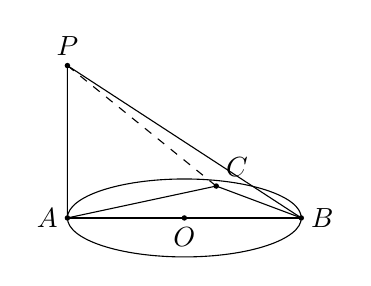
\begin{tikzpicture}[scale=0.9,>=stealth]
  \draw (0,0) ellipse (1.65 and 0.55);
  \draw[dashed] (-1.65,0)--(1.65,0);
  \draw (-1.65,0)--(1.65,0);
  \fill (0,0) circle (1.1pt) node[below] {$O$};
  \fill (-1.65,0) circle (1.1pt) node[left] {$A$};
  \fill (1.65,0) circle (1.1pt) node[right] {$B$};
  \coordinate (C) at (0.45,0.45);
  \fill (C) circle (1.1pt) node[above right] {$C$};
  \coordinate (P) at (-1.65,2.15);
  \fill (P) circle (1.1pt) node[above] {$P$};
  \draw (P)--(-1.65,0);
  \draw (P)--(1.65,0);
  \draw[dashed] (P)--(C);
  \draw (C)--(-1.65,0);
  \draw (C)--(1.65,0);
\end{tikzpicture}
\end{center}
\nopagebreak[4]
\end{question}
\begin{question}
\gkti{18}求满足方程

\nopagebreak[4]
\[
|z+3-\sqrt3i|=\sqrt3
\]

的辐角主值最小的复数 $z$。

\end{question}
\begin{question}
\gkti{19}已知抛物线

\nopagebreak[4]
\[
y^2=x+1,
\]

定点 $A(3,1)$，$B$ 为抛物线上任意一点，点 $P$ 在线段 $AB$ 上，且有 $BP:PA=1:2$。当点 $B$ 在抛物线上变动时，求点 $P$ 的轨迹方程，并指出这个轨迹为哪种曲线。

\end{question}
\begin{question}
\gkti{20}甲、乙、丙、丁四个公司承包 8 项工程，甲公司承包 3 项，乙公司承包 1 项，丙、丁两个公司各承包 2 项，问共有多少种承包方式。

\end{question}
\begin{question}
\gkti{21}已知

\nopagebreak[4]
\[
\sin A+\sin3A+\sin5A=a,
\cos A+\cos3A+\cos5A=b.
\]

求证：

（1） 当 $b\ne0$ 时，$\tan3A=\dfrac ab$；

（2） $(1+2\cos2A)^2=a^2+b^2$。

\end{question}
\begin{question}
\gkti{22}已知数列 $\{a_n\}$，其中

\nopagebreak[4]
\[
a_1=\frac43,\ a_2=\frac{13}{9},
\]

\Needspace{5\baselineskip}
且当 $n\ge3$ 时，

\nopagebreak[4]
\[
a_n-a_{n-1}=\frac13(a_{n-1}-a_{n-2}).
\]

（1） 求数列 $\{a_n\}$ 的通项公式；

（2） 求 $\displaystyle\lim_{n\to\infty}a_n$。

\end{question}